\section{Ruido y modelos determinísticos}

Denominamos ``ruido"  en un sistema de comunicaciones a una señal
que se superpone a las de interés, originada en diversas cuasas,
por ejemplo:

    \begin{itemize}
        \item agitación térmica
        \item llaves que conmutan
        \item interferencia de otros canales
    \end{itemize}
Características:
    \begin{itemize}
        \item impredecible
        \item persistente
        \item aperiódico
    \end{itemize}

\begin{figure}[htb]
    \centering\begin{minipage}{0.8\textwidth}
    \bpgf{Imagenes/ruido/ruido-1}
    \begin{tikzpicture}
        \draw[-stealth]  (-0.5,0) -- (8,0) node [anchor=north] {$t$};
        \draw[-stealth] (0,-1) -- (0,3) node [anchor=west] {$x$};
        \draw [samples=50,domain=0:7] plot (\x,{cos(\x r)+(0.5*exp(\x*0.05)-exp(-\x*0.1))+0.3*rand});
    \end{tikzpicture}
    \endpgfgraphicnamed\end{minipage}
\end{figure}
\FloatBarrier

Al diseñar el sistema de comunicación no conocemos la forma de
onda, pero es posible conocer información ``en promedio''.

\paragraph{Dos posibles modelos: }$\phantom{1}$

\begin{minipage}[t]{0.45\textwidth}
    Determinístico, promedios en el tiempo

    \begin{align*}
        \text{Valor medio:}\  \langle x \rangle &= \lim_{T\to\infty} \frac{1}{T} \int^{\frac{T}{2}}_{-\frac{T}{2}} x(t)\d t\\
        \text{Potencia media:}\ \langle x^2 \rangle &= \lim_{T\to\infty} \frac{1}{T} \int^{\frac{T}{2}}_{-\frac{T}{2}} x^2(t)\d t
    \end{align*}
\end{minipage}
\hfil
\begin{minipage}[t]{0.45\textwidth}
    Proceso aleatorio $X(t,\alpha)$, promedios ``en el ensemble'', es decir en ``sorteo'' $\alpha$.
    \begin{align*}
        \text{Valor esperado:} &\quad E \left[X(t,\alpha)\right]\\
        \mbox{}\\
        \text{Momento de orden $2$:} &\quad E \left[X^2(t,\alpha)\right]
    \end{align*}
\end{minipage}

Nos interesa obtener información \emph{espectral} sobre este tipo
de señales, pese a no disponer de una fórmula sencilla para $x(t)$
y por tanto no disponer de una transformada de Fourier.


En ese sentido, comparemos una señal de ruido como $x(t)$ de la
figura anterior con otra, %$\tilde{x}(t)$

    \begin{figure}[htb]
    \centering\begin{minipage}{0.8\textwidth}
                \bpgf{Imagenes/ruido/ruido-2}
                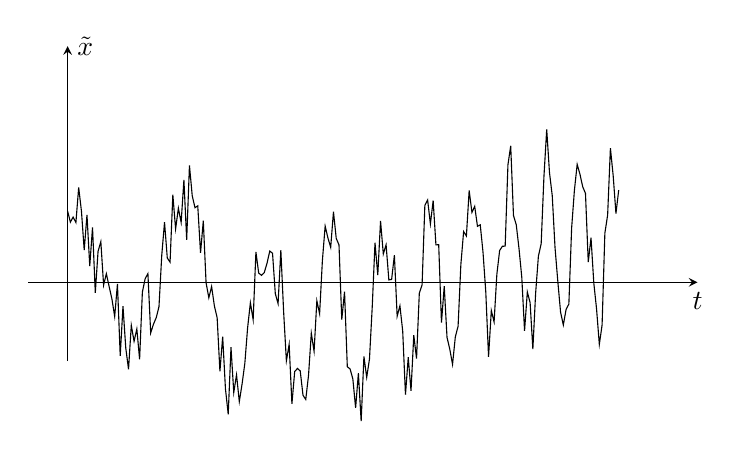
\begin{tikzpicture}
                \draw[-stealth]  (-0.5,0) -- (8,0) node [anchor=north] {$t$};
                \draw[-stealth] (0,-1) -- (0,3) node [anchor=west] {$\tilde{x}$};
                \draw [samples=200,domain=0:7] plot (\x,{cos((\x+1)^2 r)+0.5*cos(\x r)+0.5*rand});
            \end{tikzpicture}
                \endpgfgraphicnamed
             \end{minipage}
\end{figure}
\FloatBarrier

 Puede ocurrir que la potencia media sea igual en
ambas, es decir $\langle x^2\rangle = \langle \tilde{x}^2
\rangle$, pero su efecto en un sistema será en general diferente,
debido a que la segunda ``varía más rápido" en el tiempo. Por
ejemplo, a la salida de un pasabajos, $\tilde{x}$ se atenuará más,
su potencia está en ``frecuencias más altas¨. Queremos formalizar
este concepto pese a que no disponemos de una transformada de
Fourier de la propia señal.

El camino para el análisis es el estudio de la
\emph{autocorrelación} de la señal $r_x(\tau)$, y su transformada
de Fourier, la {\em densidad espectral de potencia} $S_x(f)$.
Repasamos ambos conceptos a continuación, comenzando por los
modelos determinísticos.

%
% Vemos que si bien
%tienen características bien distintas. Puede pasar que pero ambas
%no tienen el mismo efecto en un sistema. Por lo tanto importa
%poder decir cómo se distribuye esa potencia entre las distintas
%frecuencias. Esta información, la es crucial para el análisis del
%ruido.
%
%    No es fácil hallar $\hat{X}_2(f)$ para este tipo de señales. El camino para introducir $S_x(f)$ es a través de la  $x_2(t)$.


\subsection*{Modelo determinístico: señales de potencia finita}

\subsubsection*{Autocorrelación y densidad espectral de potencia}

\[r_x(\tau)=\lim_{T\rightarrow\infty} \frac{1}{T}\int^{\frac{T}{2}}_{-\frac{T}{2}} x(t)\overline{x(t-\tau)}\d t.\]

\begin{propiedadesSN}\mbox{}
    \begin{enumerate}
        \item $r_x(0)=\langle x^2\rangle$.
        \item $|r_x(\tau)|\leq r_x(0)$.
        \item $r_x(\tau) = r_x(-\tau)$ si $x(t)$ es real.
    \end{enumerate}
\end{propiedadesSN}

Un valor grande de $r_x(\tau)$ quiere decir que $x(t)$ ``tiende a
repetirse'' cada $\tau$ segundos. Entonces $r_x(\tau)$ tiene
información de tipo espectral, es decir revela las periodicidades
de la señal. Esto conduce a considerar su transformada de Fourier,

\[r_x(\tau)\stackrel{\mathcal{F}}{\longrightarrow} S_x(f)\qquad\text{densidad espectral de potencia.}\]


\begin{propiedadesSN}\mbox{}
    \begin{enumerate}
        \item $S_x(f)\geq 0$.
        \item $\langle x^2\rangle = \int^{\infty}_{-\infty} S_x(f)\d
        f$.
    \end{enumerate}
\end{propiedadesSN}

Nos dice como se distribuye la potencia en frecuencia.

\subsubsection*{Filtrado}
%
%\begin{figure}[htb]
%    \centering
%    \bpgf{Imagenes/ruido/ruido-3}
%    \begin{blockdiagram}
%        \matrix[row sep=5mm, column sep=10mm]{
%            \node[etiqueta] (inicio) {$x(t)$}; & \node[block] (filtro) {$\hat{H}(f)$} node [above=3mm] {FILTRO LTI}; & \node[etiqueta] (salida) {$y(t)$};\\
%        };
%        \draw [-stealth] (inicio) -- (filtro);
%        \draw [-stealth] (filtro) -- (salida);
%    \end{blockdiagram}
%    \endpgfgraphicnamed
%\end{figure}

Excitamos un sistema LTI, con respuesta impulsiva $h(t)$,
respuesta en frecuencia $\hat{H}(f)$, con una señal de potencia
finita $x(t)$.

\begin{figure}[h]
    \centering
\setlength{\unitlength}{0.00500in}
\begin{picture}(380,160)(140,40)
\put(220,40){\framebox(120,120){}} \put(80,100){\vector(1,0){140}}
\put(340,100){\vector(1,0){140}}
\put(0,90){\makebox(0,0)[lb]{\raisebox{0pt}[0pt][0pt]{\large $x(t)$}}}%
\put(240,90){\makebox(0,0)[lb]{\raisebox{0pt}[0pt][0pt]{\large $\hat{H}(f)$}}}%
\put(510,90){\makebox(0,0)[lb]{\raisebox{0pt}[0pt][0pt]{\large $y(t)$}}}%
\end{picture}
\end{figure}
\FloatBarrier

Se cumple:

\begin{align*}
r_y & =r_x\ast h \ast \tilde{h}\ \  \text{ donde } \ \
\tilde{h}(t)=h(-t) \\
\Rightarrow S_y(f)&=S_x(f)|\hat{H}(f)|^2.\end{align*}

\subsubsection*{Correlación y densidad espectral cruzada de dos señales}
\begin{align*}
    r_{xy}(\tau)&=\lim_{T\rightarrow\infty} \frac{1}{T}\int^{\frac{T}{2}}_{-\frac{T}{2}}x(t)\overline{y(t-\tau)}\d t.\\
    r_{xy}&=\overline{r_{yx}(-\tau)}.\\
    S_{xy}(f)&=\mathcal{F}\left[r_{xy}(\tau)\right] \text{ (no necesariamente positiva)}.\\
\end{align*}

Si $y(t)$ se obtiene de filtrar $x(t)$ como arriba:
\[ r_{xy} = r_x \ast \tilde{h},\qquad S_{xy}(f)=\overline{\hat{H}(f)} S_x(f).\]

\emph{Señales ``incoherentes'': } si $r_{xy}\equiv 0$. En ese
caso, $\langle (x+y)^2 \rangle = \langle x^2 \rangle + \langle y^2
\rangle$.

\subsubsection*{Ruido blanco}

Señal que cumple $S_n(f)\equiv \frac{\eta}{2}\,\forall\,f$. La potencia de salida de un filtro excitado por ruido blanco es
\[N=\frac{\eta}{2}\int^\infty_{-\infty}\left|\hat{H}(f)\right|^2\d f.\]

\subsection*{Aplicación: ruido en la comunicación de banda base}

\begin{figure}[htb]
    \centering\begin{minipage}{\textwidth}
    \bpgf{Imagenes/ruido/ruido-4}
    \begin{blockdiagram}
        \matrix[row sep=5mm, column sep=10mm]{
        & & \node [etiqueta] (ruido) {$n(t)$}; &\\
        \node [etiqueta] (inicio) {$x(t)$}; & \node [block] (canal) {CANAL}; & \node [operator] (sum) {$+$}; & \node [etiqueta] (salida) {$x_R(t)$};\\
        };
        \draw [-stealth] (inicio) -- (canal);
        \draw [-stealth] (canal) -- (sum);
        \draw [-stealth] (ruido) -- (sum);
        \draw [-stealth] (sum) -- (salida);
    \end{blockdiagram}
    \endpgfgraphicnamed\end{minipage}
\end{figure}
\FloatBarrier

\paragraph{Suponemos: }
\begin{itemize}
    \item $x(t)$ señal de banda acotada a $B$, potencia $\langle x^2
    \rangle$.
    \item $x_R(t) = Kx(t) + n(t)$, $n(t)$ ruido blanco,
    $S_n(f)=\frac{\eta}{2}$.
\end{itemize}

Si comparamos potencias, la señal está sumergida en ruido (de
potencia infinita!) Para mejorar las cosas agregamos un filtro
pasabajos de ancho $B$.


\begin{figure}[htb]
    \centering\begin{minipage}{\textwidth}
    \bpgf{Imagenes/ruido/ruido-3}
    \begin{blockdiagram}
        \matrix[row sep=5mm, column sep=10mm]{
            \node[etiqueta] (inicio) {$x_R(t)$ \quad }; & \node[block] (filtro) {PASABAJOS $B$}; & \node[etiqueta] (salida) {\quad $x_D(t)+n_D(t)$};\\
        };
        \draw [-stealth] (inicio) -- (filtro);
        \draw [-stealth] (filtro) -- (salida);
    \end{blockdiagram}
    \endpgfgraphicnamed\end{minipage}
\end{figure}



%
%\begin{figure}[h]
%    \centering
%\setlength{\unitlength}{0.00500in}
%\begin{picture}(380,160)(140,40)
%\put(220,40){\framebox(120,120){}} \put(80,100){\vector(1,0){140}}
%\put(340,100){\vector(1,0){140}}
%\put(-20,90){\makebox(0,0)[lb]{\raisebox{0pt}[0pt][0pt]{ $x_R(t)$}}}%
%\put(230,90){\makebox(0,0)[lb]{\raisebox{0pt}[0pt][0pt]{ $\hat{H}(f)$}}}%
%\put(510,90){\makebox(0,0)[lb]{\raisebox{0pt}[0pt][0pt]{ $x_D(t)+n_D(t)$}}}%
%\end{picture}
%\end{figure}
%\FloatBarrier

A la salida tenemos $x_D(t)=Kx(t)$ y un ruido $n_D(t)$ de potencia
media
\[\langle n_D^2 \rangle = \int^\infty_{-\infty} S_{n_D}(f)\d f =
\frac{\eta}{2}\int^\infty_{-\infty}\left|\bar{H}(f)\right|^2\d f=
\eta B.\]

Por lo tanto, relación señal - ruido a la salida es
\[
\left(\frac{S}{N}\right)_D= \dfrac{K^2\langle x^2 \rangle}{\eta
B}.\]
